\documentclass{article}
\usepackage[utf8]{inputenc}
\usepackage{multicol}
\usepackage{listings}
\usepackage{verbatim}
\usepackage{color}
\usepackage{geometry}
\usepackage{float}
\usepackage{amsmath}

\usepackage{pdflscape}
\usepackage{hyperref}
\setlength{\belowcaptionskip}{-10pt}
\setlength{\abovecaptionskip}{-30pt}
\floatstyle{boxed} 
\restylefloat{figure}
\usepackage{graphicx}
\definecolor{codegreen}{rgb}{0,0.6,0}
\definecolor{codegray}{rgb}{0.5,0.5,0.5}
\definecolor{codepurple}{rgb}{0.58,0,0.82}
\definecolor{backcolour}{rgb}{0.95,0.95,0.92}

\lstdefinestyle{mystyle}{
	backgroundcolor=\color{backcolour},   
	commentstyle=\color{codegreen},
	keywordstyle=\color{blue},
	numberstyle=\tiny\color{codegray},
	stringstyle=\color{codepurple},
	basicstyle=\footnotesize,
	breakatwhitespace=false,         
	breaklines=true,                 
	captionpos=b,                    
	keepspaces=true,                 
	numbers=left,                    
	numbersep=5pt,                  
	showspaces=false,                
	showstringspaces=false,
	showtabs=false,                  
	tabsize=2
}

\lstset{style=mystyle}
\title{Data Mining\\
		Home work 07\\Association rules, }
\author{Aqeel Labash\\ \textbf{Lecturer:} Jaak Vilo}
\date{23 March 2016}

\geometry{
	a4paper,
	total={170mm,257mm},
	left=10mm,
	top=5mm,
}
\begin{document}
	\maketitle
\section*{First Question}
For this task I used \textbf{arule} library. Specifically the functions \textbf{apriori, eclat}.\\
\textbf{apriori:} get list of rules.\\
\textbf{eclat:} get list of item sets.\\
both of them need optional  parameters (support , minimum length , only apriori :confidence ).\\
Only apriori need appearance as optional option which determine lhs or rhs for the rules.\\
The code I used is here :
\begin{lstlisting}[language=R]
###First Question ####
library(arules)
supermarket = read.transactions('supermarket.txt',format = 'basket',sep=" ")
tim = proc.time()
rules = apriori(supermarket,parameter = list(minlen=2,supp = 0.01,conf=0.05))#,conf=0.5))
print (proc.time()-tim)
tim = proc.time()
itmset = eclat(supermarket,parameter = list(supp = 0.01, maxlen = 15))
print (proc.time()-tim)
inspect(itmset)
head(inspect(rules))
head(inspect(itmset))
?apriori
?eclat
\end{lstlisting}
I selected a low confidence to get more rules because raising it will decrease them (choose least number came to my mind).\\
Here is the head of rules :\\
\begin{tabular}{|c*{6}{|c}}
	\hline
&lhs&rhs&support&confidence&lift\\
\hline
1&{14914}&{5330}&0.01111024&0.89240506&4.568581\\
\hline
2&{5330}&{14914}&0.01111024&0.05687777&4.568581\\
\hline
3&{12562}&{5330}&0.01623198&0.86736842&4.440408\\
\hline
4&{5330}&{12562}&0.01623198&0.08309802&4.440408\\
\hline
5&{11995}&{5330}&0.01591679&0.76226415&3.902337\\
\hline
6&{5330}&{11995}&0.01591679&0.08148447&3.902337\\
\hline
\end{tabular} \\ \\
Here is the head of item sets :\\ \\
\begin{tabular}{|c*{3}{|c}}
	\hline
&items&support\\
	\hline
1&{14914,5330}&0.01111024\\
	\hline
2&{12562,5330}&0.01623198\\	\hline
3&{11995,5330}&0.01591679\\	\hline
4&{6385,9108}&0.01193759\\	\hline
5&{5330,6385}&0.01012529\\	\hline
6&{4037,9108}&0.01079505\\ 	\hline
\end{tabular}

Apriori used 0.156 sec.
eclat used 0.158 sec.
\section*{Second Question}
For this task I used the following code to get top of every list:\\
\begin{lstlisting}[language=R]
high.support<- sort(rules, decreasing = TRUE, na.last = NA, by = "support")
high.confidence<- sort(rules, decreasing = TRUE, na.last = NA, by = "confidence")
high.lift<- sort(rules, decreasing = TRUE, na.last = NA, by = "lift")
\end{lstlisting}
After that I used this code to build the contingency matrix for every rule.Kinda a straight forward solution (brute force).
\begin{lstlisting}[language=R]

#### Second Question #####
high.support<- sort(rules, decreasing = TRUE, na.last = NA, by = "support")[1:10,]
high.confidence<- sort(rules, decreasing = TRUE, na.last = NA, by = "confidence")[1:10,]
high.lift<- sort(rules, decreasing = TRUE, na.last = NA, by = "lift")[1:10,]
lst<-read.csv('supermarket.txt',header = FALSE,sep=" ")

FindAllInfoV2 <- function(rule, dataset){
# Extract the left hand side of the rule
lhs.tbl <- itemInfo(lhs(rule))[which(as(lhs(rule), "matrix")[1, ] == 1), ]
rhs.tbl <- itemInfo(rhs(rule))[which(as(rhs(rule), "matrix")[1, ] == 1), ]
TP = 0
TN= 0 
FP =0
FN = 0

for(i in seq_len(nrow(dataset)))
{
#Left Hand exist
l <- sum(lhs.tbl %in% dataset[i,])
r <- sum(rhs.tbl %in% dataset[i,])
l <- l>=length(lhs.tbl)
r <- r>=length(rhs.tbl)
if (l)
{
#right hand also exist
if (r)
{
TP<-TP+1
}
else
{
FN<-FN+1
}
}
#left hand doesn't exist
else
{
#but right hand exist
if (r)
{
FP<-FP+1
}
#also right hand doesn't exist
else
{
TN<-TN+1
}
}
}
leftside =0
if (length(lhs.tbl)>1)
{
leftside = paste(lhs.tbl, collapse = ',')
}
else
{
leftside = strtoi(lhs.tbl, base = 0L)
}
return (c(quality(rule)[1],quality(rule)[2],quality(rule)[3],left =leftside,right =strtoi(rhs.tbl, base = 0L),F11= TP,F10=FN,F01=FP,F00=TN))
}
dfsupport<- data.frame()
for (i in seq_len(length(high.support)))
{
dfsupport<-rbind(dfsupport,FindAllInfoV2(high.support[i],lst))
}

dfconfidence<- data.frame()
for (i in seq_len(length(high.confidence)))
{
dfconfidence<-rbind(dfconfidence,FindAllInfoV2(high.confidence[i],lst))
}
dflift<-data.frame()
for (i in seq_len(length(high.lift)))
{
dflift<-rbind(dflift,FindAllInfoV2(high.lift[1],lst))
}
dfsupport
dfconfidence
dflift
\end{lstlisting}
The previous code will build 3 tables for the top support,lift,confidence between the rules we found.\\
Support table :\\
\begin{tabular}{|l|*{9}{c|}}
	\hline
N&support&confidence&lift&left&right&F11&F10&F01&F00\\
\hline
1&0.06973446&0.3569988&1.626812&5330&9108&1396&3562&4174&23428\\
\hline
2&0.06973446&0.3177738&1.626812&9108&5330&1396&4174&3562&23428\\
\hline
3&0.02935151&0.3755040&1.711139&13973&9108&449&1535&5121&25455\\
\hline
4&0.02935151&0.1337522&1.711139&9108&13973&449&5121&1535&25455\\
\hline
5&0.02907572&0.2940239&1.339841&11217&9108&538&1972&5032&25018\\
\hline
6&0.02907572&0.1324955&1.339841&9108&11217&538&5032&1972&25018\\
\hline
7&0.02718462&0.2749004&1.407326&11217&5330&357&2153&4601&25449\\
\hline
8&0.02718462&0.1391690&1.407326&5330&11217&357&4601&2153&25449\\
\hline
9&0.02671184&0.2833264&1.291093&14155&9108&377&2016&5193&24974\\
\hline
10&0.02671184&0.1217235&1.291093&9108&14155&377&5193&2016&24974\\
\hline
\end{tabular}\\\\
The Confidence table :\\ 
\begin{tabular}{|l|*{9}{c|}}
	\hline
N&support&confidence&lift&left&right&F11&F10&F01&F00\\
\hline
1&0.01111024&0.8924051&4.568581&14914&5330&137&179&4821&27423\\
\hline
2&0.01623198&0.8673684&4.440408&12562&5330&308&167&4650&27435\\
\hline
3&0.01591679&0.7622642&3.902337&11995&5330&275&255&4683&27347\\
\hline
4&0.01296194&0.5007610&2.281924&13973,5330&9108&125&178&5445&26812\\
\hline
5&0.01296194&0.4416107&2.260783&13973,9108&5330&125&324&4833&27278\\
\hline
6&0.02194469&0.4258410&1.940520&3723&9108&407&901&5163&26089\\
\hline
7&0.01386810&0.4141176&1.887098&4185&9108&226&624&5344&26366\\
\hline
8&0.02450556&0.4005151&1.825112&3423&9108&499&1054&5071&25936\\
\hline
9&0.01028288&0.3782609&1.723702&11217,5330&9108&101&256&5469&26734\\
\hline
10&0.02935151&0.3755040&1.711139&13973&9108&449&1535&5121&25455\\
\hline
\end{tabular}\\ \\ 
The top lift table : \\
\begin{tabular}{|l|*{9}{c|}}
	\hline
N&support&confidence&lift&left&right&F11&F10&F01&F00\\\hline
1&0.01111024&0.89240506&4.568581&14914&5330&137&179&4821&27423\\\hline
2&0.01111024&0.05687777&4.568581&5330&14914&137&4821&179&27423\\\hline
3&0.01623198&0.86736842&4.440408&12562&5330&308&167&4650&27435\\\hline
4&0.01623198&0.08309802&4.440408&5330&12562&308&4650&167&27435\\\hline
5&0.01591679&0.76226415&3.902337&11995&5330&275&255&4683&27347\\\hline
6&0.01591679&0.08148447&3.902337&5330&11995&275&4683&255&27347\\\hline
7&0.01063746&0.20642202&3.373731&3723&3423&267&1041&1286&29966\\\hline
8&0.01063746&0.17385705&3.373731&3423&3723&267&1286&1041&29966\\\hline
9&0.01036167&0.20107034&2.572363&3723&13973&107&1201&1877&29375\\\hline
10&0.01036167&0.13256048&2.572363&13973&3723&107&1877&1201&29375\\\hline
\end{tabular}
\section*{Third Question}
For this task I think actually Jaccard measurement could help. \(\zeta = \frac{P(A\cap B)}{P(A)+P(B)-P(A\cap B)}\).With this measurement we can know how much the rule predict a correct answer.
To calculate Jaccard value I used the following code :

\begin{lstlisting}[language=R]
###### Third Question #####

calculatelaplace<-function(thedata)
{
#Jaccard = f11/f1plus+fplus1-f11
#fplus1= f11+f01
#f1plus= f11+f10
thedata$Jaccard <- thedata$F11/(thedata$F11+thedata$F01+thedata$F10)
return (thedata)
}
dfsupport<-calculatelaplace(dfsupport)
dflift<-calculatelaplace(dflift)
dfconfidence<-calculatelaplace(dfconfidence)
for (i in seq_len(10))
{

print (c(i,dfsupport$Jaccard[i],dfconfidence$Jaccard[i],dflift$Jaccard[i]))
}
\end{lstlisting}
In the following table we can see Jaccard measurment for the previous 3 lists (linked by row number):\\
\begin{tabular}{|l|*{4}{c|}}\hline
Number&Sup\_Jac&Confid\_Jac&Lift\_Jac\\ \hline
1&0.15286903&0.02666926&0.02666926\\\hline
2&0.15286903&0.06009756&0.02666926\\\hline
3&0.06319493&0.05275273&0.06009756\\\hline
4&0.06319493&0.02174669&0.06009756\\\hline
5&0.07133386&0.02366528&0.05275273\\\hline
6&0.07133386&0.06289600&0.05275273\\\hline
7&0.05020391&0.03648692&0.10292984\\\hline
8&0.05020391&0.07533213&0.10292984\\\hline
9&0.04969681&0.01733608&0.03359498\\\hline
10&0.04969681&0.06319493&0.03359498\\ \hline
\end{tabular}
\section*{Fourth Question}
Actually there is so many things coming to my mind.
\begin{enumerate}
	\item We can see what people buy in general in specific time.
	\item what's the most bought items in certain area.
	\item Most bought items together.
	\item Detect approximate area for customer (home , work) depending on his usual buying location and products.
	\item Find what type of the area around the shop depending on the most bought items (resident , companies, sports ..).
	\item Specify customer (married , single ) depending on frequent products bought.
	\item Specify customer gender depending on frequent items bought.
\end{enumerate}
\section*{Fifth Question}
In this tasked I picked the first rule in support table where it's contingency table looks like the following : \\
\begin{tabular}{|l|*{3}{c|}}
	\hline
&9108&not 9108 \\ \hline
5330&F11=1396&F10 = 3562\\ \hline
not 5330&F01=4174&F00= 23428 \\ \hline
\end{tabular}
\textbf{Total:}32560 transaction.Now to calculate \(P(A|B)\) we use the formula :\[P(A|B)=\frac{P(A\cap B)}{P(B)}\] Where\(A\) is "5330" and \(B\) is "9108".
\[P(B) = \frac{1396+4174}{32560},P(A\cap B)=\frac{1396}{32560}\Longrightarrow P(A|B) = \frac{\frac{1396}{32560}}{\frac{5570}{32560}}=\frac{1396}{5570} \simeq 0.25\]
To calculate \(P(B|A)\) we can use Bayes rule.Firstly the description of how we come with Bayes rule, after that we use the rule.
\[P(A|B) = \frac{P(A\cap B)}{P(B)}\Longrightarrow P(A\cap B) = P(A|B)P(B) \]
\[P(B|A) = \frac{P(A\cap B)}{P(A)}\Longrightarrow P(A\cap B) = P(B|A)P(A) \]
From the previous two formulas we get : 
\[P(A|B)P(B) = P(B|A)P(A) \Longrightarrow P(B|A) = \frac{P(A|B)P(B)}{P(A)}\]
Which is the Bayes rule.
\[P(A) = \frac{1396+3562}{32560} = \frac{4958}{32560}\]
\[P(B|A) = \frac{0.25* 4958}{5570}\simeq 0.22 \]
\section*{Sixth Question}
For this task I did the following :
\begin{enumerate}
	\item I tried to run but didn't work so I built it again following the commands in \href{https://courses.cs.ut.ee/MTAT.03.183/2016_spring/uploads/Main/krimp_compilation.txt}{this link}
	\item copied krimp file to bin folder where all the configuration exist.
	\item changed datadir.conf folders to fit linux.
	\item changed fic.conf to point to supermarket(conf) file instead of compress(conf)
	\item modified fic.user.conf so the application can use up to 4GB of ram instead of 1GB.
	\item copied supermarket.txt to dataset folder and changed the suffix to dat.
	\item modified convertdb.conf.Changed dbName value to supermarket.After that executed krimp with convertd.conf to convert my file to db by the command krimp convertdb.conf
	\item I replicated compress file changed the file name ,unhashed the dataType = bai32 because uint8 and bm128 wasn't able to handle more than 128 item (our database have more than 15k item).
	\item Done many experiments with threads number but all the threads worked on the same core so I changed it to single thread.
	\item I built a python code to get a specific number of items+ one line items.
	\item I used 127 and got about 133 item. started the application at 12:40 AM 25-Mar which didn't work.
\end{enumerate}
Here is the python code I used to generate the new file:
\begin{lstlisting}[language=Python]
import numpy as np
#read file
f = open ('supermarket.txt')
lines = f.readlines()

#Set around max number of items
breakpoint = 127
t = set()
def AddElements(line):
elements = line.split(" ")
for element in elements:
t.add(element.strip())

#Shuffle the lines to get random lines.
np.random.shuffle(lines)
outputfile=[]

#Write Selected lines to file
def WriteToFile():
output = open('supermarket.dat','w')
for l in outputfile:
output.write(l)

#Add lines
for line in lines:
outputfile.append(line)
AddElements(line)
if len(t)>breakpoint:
break

#Write lines to file
WriteToFile()
\end{lstlisting}
Next day morning I woke up on this error :
\begin{lstlisting}
** Processing conf: 'fic.conf'
* Verbosity:		2
* Max Mem Usage:	4096mb
* Priority:		Opzij, opzij, opzij!
Maak plaats, maak plaats, maak plaats!
Wij hebben ongelovelijke haast!

** Database :: 
* File:		supermarket.db
* Database:		19t 19r, 154i, 1066.07bits
* 			pruned below support 0, maximum set length 39
* Alphabet:		133 items
* Internal datatype:	32bit bitmap array

** ItemSetCollection ::
* Mining:		Storing chunk #177             
!! Run-time fatal exception:
! WriteItemSet - Error writing ItemSet
\end{lstlisting}
It took about 60GB and left about 137 MB of hard disk drive.
\begin{figure}[H]
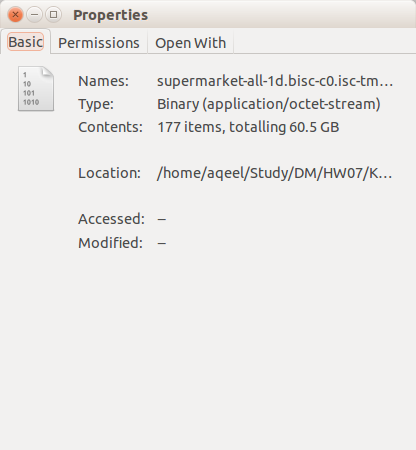
\includegraphics[scale=1]{size.png}
\end{figure}
\begin{figure}[H]
	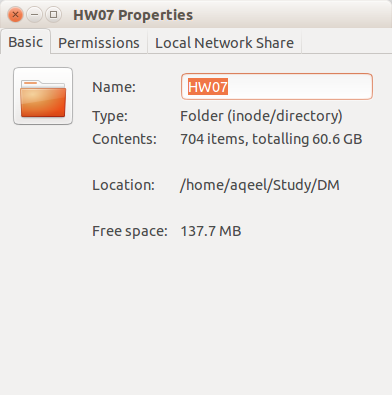
\includegraphics[scale=1]{space.png}
\end{figure}
The previous try took about 9 hours from around 12~ to 8:49.
Tried to play with parameters but nothing worked out at least for me.\\ And I raise my case:)\\
Link to files :.R,.ipython,.py,.tex,.pdf can be found \href{https://github.com/aqeel13932/DM/tree/master/HW07}{here}
\begin{center}
\textbf{E.O.F}
\end{center}

\end{document}